\chapter{Etude de l'existant}
\section{Introduction}
    L'étude de l'existant est une phase cruciale dans le domaine des systèmes d'information,
    où l'on examine en détail tous les éléments qui composent le système actuel.\\
    Cette démarche vise à rassembler un maximum d'informations pertinentes concernant 
    le domaine d'étude afin de mettre en lumière les problèmes et les défis auxquels le système actuel est confronté.\\
    En comprenant les mécanismes et les rouages de la situation présente, 
    on se dote des outils nécessaires pour proposer des solutions efficaces et adaptées.\\
    L'étude de l'existant implique une analyse approfondie des processus, des flux de données,
    des technologies mises en œuvre et des interactions entre les acteurs impliqués.\\
    Cette démarche permet de dresser un état des lieux objectif et exhaustif,
    mettant en évidence les forces et les faiblesses du système actuel.\\
    L'objectif ultime de cette étude est d'identifier les points de blocage, 
    les inefficacités et les goulots d'étranglement susceptibles d'entraver le bon fonctionnement du système d'information.\\
    En comprenant ces problèmes, les professionnels du domaine peuvent alors concevoir des solutions adaptées, 
    innovantes et pérennes pour améliorer l'efficacité, la performance et la sécurité du système.\\
\section{Flux d’information}
    \subsection{Définition}
        désigne la circulation ou le déplacement de l'information d'un endroit à un autre au sein d'un système, 
        d'une organisation ou entre différentes entités. \\
        Il se caractérise par plusieurs aspects essentiels:
        \begin{itemize}
            \item Champ de départ: Il s'agit de la source ou de l'origine de l'information, c'est-à-dire l'endroit où l'information est créée ou initiée. Cela peut être une personne, un département, un système informatique, ou toute autre source d'information.
            \item Champ d'arrivée: C'est le destinataire ou le récepteur de l'information, c'est-à-dire l'endroit où l'information est destinée à être utilisée ou traitée. Comme pour le champ de départ, cela peut être une personne, un groupe, un système informatique, etc.
            \item Nature de l'information: Ce paramètre définit le type ou la catégorie de l'information en circulation. Il peut s'agir de données numériques, de textes, d'images, de vidéos, de fichiers, de rapports, etc. La nature de l'information influence souvent le mode de traitement et de transmission utilisé.
            \item Volume de l'information: Le volume représente la quantité ou la taille de l'information en transit. Cela peut varier considérablement, allant de petites quantités de données à de grandes quantités de données, en fonction des besoins spécifiques du système ou des processus en cours.
        \end{itemize}
    \subsection{Diagramme du flux d’Information}
        Le formalisme de ce diagramme est simple les parties prenantes sont
        représentées par des symboles en suivant la logique suivante:l'acteur (champs
        d'étude) est représenté par un carre, les postes internes à l'entreprise sont
        représentés par des éclipses, le poste externe à l'entreprise par un cadre, tandis
        que les informations (Flux) par des flèches numérotées.
    \subsection{La légende du flux d’information}
        \begin{figure}[H]
            \centering
            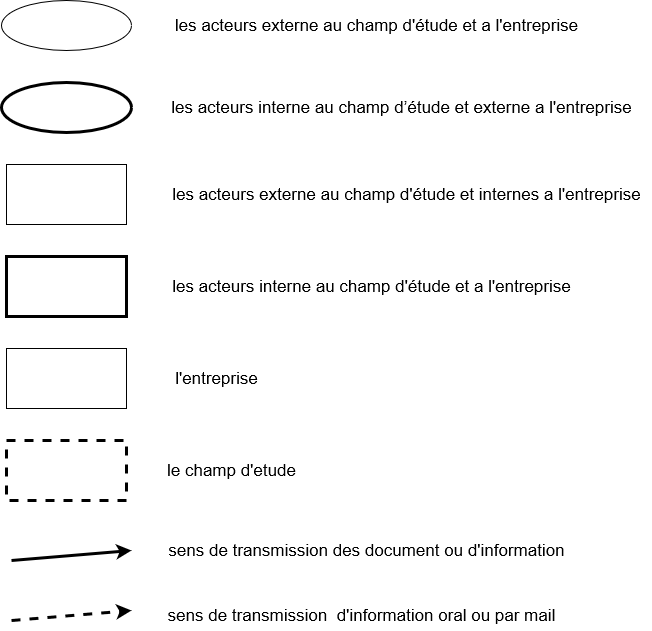
\includegraphics[width=0.8\textwidth]{images/legende.png}
            \caption{La légende du flux d’information}
            \label{fig:La légende du flux d’information}
        \end{figure}
        \newpage
    \subsection{Flux d’information}
        \begin{figure}[ht!]
            \centering
            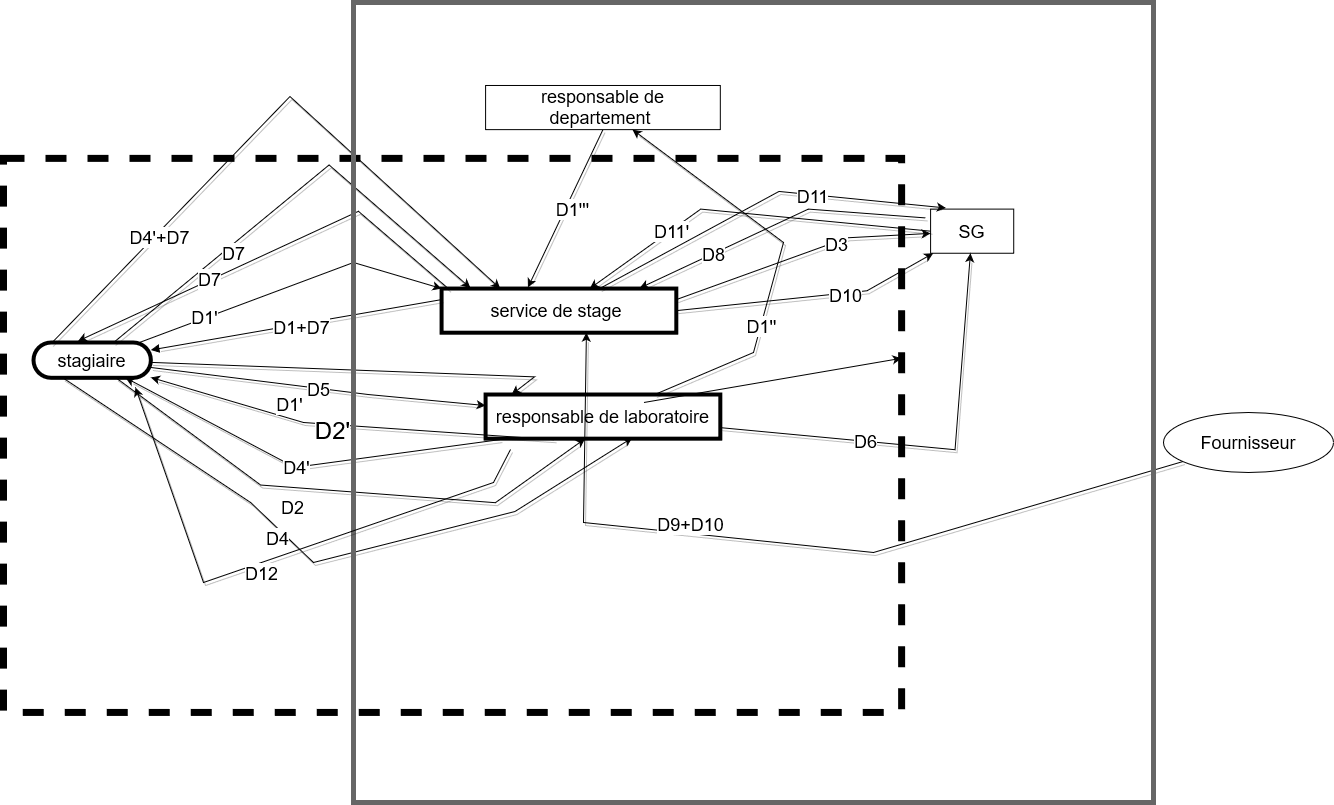
\includegraphics[width=0.8\textwidth]{images/Flux.png}
            \caption{Diagramme  du Flux d'Information}
            \label{fig:Diagramme  du Flux d'Information}
        \end{figure}
\subsection{Description du flux d'information}
\begin{itemize}
    \item D1:fiche de stage 
    \item D1':fiche de stage rempli par stagiaire
    \item D1'':fiche de stage signier par responsable de laboratoire 
    \item D1''':fiche de stage signier par responsable de departement 
    \item D2:rapport d'expérience 
    \item D2':rapport d'expérience signer
    \item D3:demande d'achat 
    \item D4:demande de produit et verrerie 
    \item D4': demande de produit et verrerie signier par responsable de laboratoire 
    \item D5: demande d'analyse 
    \item D6:demande de maintenance 
    \item D7: carte de stagiaire 
    \item D8:bon de commande 
    \item D9:bon de livraison 
    \item D10:facture 
    \item D11:fiche d inventaire
    \item D11':fiche d inventaire signier par SG
    \item D12: rendez-vous
\end{itemize}

\section{Etude des Postes de Travailles}
\subsection{Définition}
Un poste de travail est un lieu ou une ou plusieurs personnes effectuent un
certain nombre de taches par les ressources dont elle dispose.\\
Les postes de travail sont parmi les points essentiels pour le traitement de
l'information.
\subsection{Les Poste de Travail}

\newpage

\begin{center}
\Huge FICHE ETUDE DE POSTE
\end{center}

\vspace{0.5cm}
    


\begin{flushleft}
\textbf{Désignation poste:} Stagiaire \\
\textbf{Service de rattachement:} / \\
\textbf{Effectif:} 8 \\
\textbf{Moyens de traitement:} papier,stylo \\

\vspace{1cm}

\textbf{Les tâches accomplies par ce poste:}\\
\begin{itemize}
    \item remplire Fiche de Stage
    \item edition de Demande de Produit et Verrerie
    \item edition de Demande d'analyse
    \item edition de Rapport d'Expérience
    \item Mise à jour de le Registre des résultats
\end{itemize}

\end{flushleft}

\vspace{1cm}

Les documents entrants à ce poste :

\begin{table}[ht]
\begin{tabularx}{\textwidth}{|*{4}{>{\centering\arraybackslash}X|}}
  \hline
  \textbf{Emetteur} & \textbf{Désignation} & \textbf{Nbre exemplaire}  & \textbf{Fréquence} \\
  \hline
  service de stage & Fiche de Stage & 1 & Debut de Stage  \\
  service de stage &  carte de stagiaire & 1 & Debut de Stage  \\
  Responsable de laboratoire & mail de rendez-vou & 1 & Aléatoire \\
  Responsable de laboratoire & Rapport d'Expérience signé & 2 & Aléatoire \\
  \hline
\end{tabularx}
\end{table}

\vspace{1cm}

Les documents remplis et crées par ce poste :

\begin{table}[ht]
\begin{tabularx}{\textwidth}{|*{3}{>{\centering\arraybackslash}X|}}
  \hline
  \textbf{Désignation } & \textbf{Nbre exemplaire} & \textbf{Fréquence} \\
  \hline
  Fiche de Stage & 1 & Debut de Stage\\
  Demande de Produit et Verrerie & 1 & Aléatoire  \\
  Demonde d'analyse & 1 & Aléatoire  \\
  Rapport d'expériences & 1 & Aléatoire \\
  \hline
\end{tabularx}
\end{table}

\vspace{1cm}

Les documents sortants :

\begin{table}[ht]
\begin{tabularx}{\textwidth}{|*{4}{>{\centering\arraybackslash}X|}}
  \hline
  \textbf{Récepteur} & \textbf{Désignation} & \textbf{Nbre exemplaire}  & \textbf{Fréquence} \\
  \hline
  Responsable de laboratoire & Fiche de Stage & 1 & Debut de Stage\\
  Service de Stage & carte de Stage & 1 & Debut de Stage\\
  Service de Stage & Demande de Produit et Verrerie & 1 & Aléatoire\\
  Responsable de laboratoire & Demonde d'analyse & 1 & Aléatoire\\
  Responsable de laboratoire & Rapport d'expériences & 2 & Aléatoire \\
  \hline
\end{tabularx}
\end{table}

\vspace{1cm}


\newpage

\begin{center}
\Huge FICHE ETUDE DE POSTE
\end{center}

\vspace{0.5cm}
    


\begin{flushleft}
\textbf{Désignation poste:} Service de Stage \\
\textbf{Service de rattachement :} cellule de Stages \\
\textbf{Effectif :} 3 \\
\textbf{Moyens de traitement :} pc imprimante \\

\vspace{1cm}

\textbf{Les tâches accomplies par ce poste :}\\
\begin{itemize}
    \item Fournir les fiche de stage au stagiaire
    \item L'édition de la carte de stage
    \item modification de fiche de stage
    \item Fournir les les produit chimique au stagiaire
    \item edition de demande d'Achat
    \item modification de la fiche de stock
    \item reception des produit chimique avec bon de livraison et transmission les facture au secretaire generale
\end{itemize}

\end{flushleft}

\vspace{1cm}

Les documents entrants à ce poste :

\begin{table}[ht]
\begin{tabularx}{\textwidth}{|*{4}{>{\centering\arraybackslash}X|}}
  \hline
  \textbf{Emetteur} & \textbf{Désignation} & \textbf{Nbre exemplaire}  & \textbf{Fréquence} \\
  \hline
  Responsable de Département & Fiche de stage & 1 & Debut de Stage  \\
  stagiaire & Demande de produit et Verrerie & 1 & Aléatoire \\
  stagiaire & carte stagiaire & 1 & Aléatoire \\
  Fournisseur & bon de livraison & 1 & Aléatoire\\
  Fournisseur & Facture & 1 & Aléatoire\\
  SG & bon de commande &  1 & Aléatoire \\
   stagiaire & fiche de stage modifier & 1 &  Aléatoire\\
  \hline
\end{tabularx}
\end{table}

\vspace{1cm}

Les documents remplis et crées par ce poste :

\begin{table}[ht]
\begin{tabularx}{\textwidth}{|*{3}{>{\centering\arraybackslash}X|}}
  \hline
  \textbf{Désignation } & \textbf{Nbre exemplaire} & \textbf{Fréquence} \\
  \hline
  la carte de stage & 1 & Aléatoire \\
  Fiche de Stock & 1 & Aléatoire  \\
  demande d'Achat & 1 & Aléatoire  \\
  fiche dinventaire & 1 & Aléatoire\\
  \hline
\end{tabularx}
\end{table}

\vspace{1cm}

Les documents sortants :

\begin{table}[ht]
\begin{tabularx}{\textwidth}{|*{4}{>{\centering\arraybackslash}X|}}
  \hline
  \textbf{Récepteur} & \textbf{Désignation} & \textbf{Nbre exemplaire}  & \textbf{Fréquence} \\
  \hline
  stagiaire & Fiche de stage & 1 & Debut de Stage  \\
  stagiaire & carte de stagiaire & 1 & Aléatoire  \\
  secretaire generale & demande d'Achat & 1 & Aléatoire  \\
  secretaire generale & facture & 1 & Aléatoire  \\

  \hline
\end{tabularx}
\end{table}

\vspace{1cm}


\newpage

\begin{center}
\Huge FICHE ETUDE DE POSTE
\end{center}

\vspace{0.5cm}
    


\begin{flushleft}
\textbf{Désignation poste:} responsable de laboratoire \\
\textbf{Service de rattachement:}  Département \\
\textbf{Effectif:} 5 \\
\textbf{Moyens de traitement:} pc imprimante \\

\vspace{1cm}

\textbf{Les tâches accomplies par ce poste :}\\
\begin{itemize}
    \item signature de fiche de stage
    \item edition de demande de Maintenance
    \item mis a jour Registre de Maintenance
    \item mis a jour le Registre des rendez-vou
    \item envoyer les e-mail de rendez-vou
\end{itemize}

\end{flushleft}

\vspace{1cm}

Les documents entrants à ce poste :

\begin{table}[ht]
\begin{tabularx}{\textwidth}{|*{4}{>{\centering\arraybackslash}X|}}
  \hline
  \textbf{Emetteur} & \textbf{Désignation} & \textbf{Nbre exemplaire}  & \textbf{Fréquence} \\
  \hline
  stagiaire &  fiche de Stage & 1 &  Aléatoire \\
  stagiaire &  demandede produit et Verrerie & 1 &  Aléatoire \\
  stagiaire &  demandede danalyse & 1 &  Aléatoire \\
  stagiaire &  Rapport d expériences & 2 &  Aléatoire \\
  SG  & bon de commande & 1 &  Aléatoire \\

  \hline
\end{tabularx}
\end{table}

\vspace{1cm}

Les documents remplis et crées par ce poste :

\begin{table}[ht]
\begin{tabularx}{\textwidth}{|*{3}{>{\centering\arraybackslash}X|}}
  \hline
  \textbf{Désignation } & \textbf{Nbre exemplaire} & \textbf{Fréquence} \\
  \hline
  demande de maintenance  & 1  & Aléatoire\\
  Registre DE Maintenance  & 1  & Aléatoire\\
  \hline
\end{tabularx}
\end{table}

\vspace{1cm}

Les documents sortants :

\begin{table}[ht]
\begin{tabularx}{\textwidth}{|*{4}{>{\centering\arraybackslash}X|}}
  \hline
  \textbf{Récepteur} & \textbf{Désignation} & \textbf{Nbre exemplaire}  & \textbf{Fréquence} \\
  \hline
  Responsable de Departement &  fiche de Stage & 1 &  Aléatoire \\
  Stagiaire &  rendez-vous & 1 &  Aléatoire \\
  Stagiaire &  Rapport d expériences signé & 2 &  Aléatoire \\
  Stagiaire &   Demande de produit et Verrerie signé & 1 &  Aléatoire \\
  secretaire generale  &  demande de maintenance & 1 &  Aléatoire \\
  secretaire generale  &  facture & 1 &  Aléatoire \\
  \hline
\end{tabularx}
\end{table}

\vspace{1cm}

\section{Etude des documents}
\subsection{Définition}
Les documents sont des renseignements écrits ou objets servant de preuve
d’information ou de témoignage concernant le domaine d'étude.
L'étude des documents permet de connaitre le rôle de chaque document, son
utilité, les postes de travail qui l'utilisent et de détecter les failles et les sources
de disfonctionnement du système existant.
\subsection{Etude des documents existant}


\newpage

\begin{center}
\Huge FICHE ANALYTIQUE DE DOCUMENT
\end{center}

\vspace{0.5cm}
    

\begin{flushleft}
\textbf{Code document :} / \\
\textbf{Désignation document :} Fiche de Stage \\
\textbf{Rôle :} Il contient les informations, le matériel et les matières du stagiaire dont il a bénéficié \\
\textbf{Caractéristiques:} papier a4\\
\end{flushleft}

\vspace{1cm}

\begin{table}[ht]
\begin{tabularx}{\textwidth}{|X|X|}

\hline
\textbf{Entête(o /n) :}  o   & \textbf{fréquence:} Aléatoire  \\
\hline
\textbf{Rempli par :}  service de stages    & \textbf{Exemplaire :} 01  \\
\hline
\end{tabularx}
\end{table}

\vspace{1cm}

\begin{table}[ht]
\begin{tabularx}{\textwidth}{|X|X|X|}
  \hline
  \multicolumn{1}{|c|}{\centering\textbf{Emetteur}} & \multicolumn{1}{c|}{\centering\textbf{Récepteur}} & \multicolumn{1}{c|}{\centering\textbf{Archivage}} \\
  \hline
  service de stage & stagier  & / \\
  \hline
  stagier & Responsable du laboratoire  & / \\
  \hline
  Responsable du laboratoire & Responsable de Departement & / \\
  \hline
  Responsable de Departement & service de stage  & service de stages \\
  \hline
\end{tabularx}
\end{table}

\vspace{1cm}

\begin{table}[ht]
\begin{tabularx}{\textwidth}{|*{5}{>{\centering\arraybackslash}X|}}
  \hline
  \textbf{Rubrique} & \textbf{Type} & \textbf{Taille} & \textbf{Nature} & \textbf{Observation} \\
  \hline
  Encadrant & A & 50 & PP & / \\
  Tel Encadrant & N & 10 & PP & / \\
  Departement & A & 30 & PP & / \\
  laboratoire & A & 100 & PP & / \\
  Responsable du laboratoire & A & 50 & PP & / \\
  Specialite étudiante & A & 50 & NPP & / \\
  Theme & A & 150 & NPP & / \\
  Photo & S & / & PP & / \\
  nom & A & 25 & PP & / \\
  prenom & A & 25 & PP & / \\
  Matricule & N & 12 &  PP & / \\
  mail & AN & 100 & PP & .....@....\\
  Tel & N & 10 & PP & / \\
  Désignation verrerie & AN & 50 & PP & / \\
  QD verrerie & N & 02 & PP & / \\ 
  QR verrerie & N & 02 & PP & / \\ 
  Désignation produit  & AN & 50 & PP & / \\
  QD produit  & N & 02 & PP & / \\ 
  QR produit  & N & 02 & PP & / \\ 
  \hline
\end{tabularx}
\end{table}

\vspace{1cm}





\newpage

\begin{center}
\Huge FICHE ANALYTIQUE DE DOCUMENT
\end{center}

\vspace{0.5cm}
    

\begin{flushleft}
\textbf{Code document :} / \\
\textbf{Désignation document :} carte stagiaire \\
\textbf{Rôle :} Il contient les informations du stagiaire et prouve son affiliation \\
\textbf{Caractéristiques:} papier cartonnée a6 \\
\end{flushleft}

\vspace{1cm}

\begin{table}[ht]
\begin{tabularx}{\textwidth}{|X|X|}

\hline
\textbf{Entête(o /n) :}  o   & \textbf{fréquence:} Aléatoire  \\
\hline
\textbf{Rempli par :}  service de stage    & \textbf{Exemplaire :} 02  \\
\hline
\end{tabularx}
\end{table}

\vspace{1cm}

\begin{table}[ht]
\begin{tabularx}{\textwidth}{|X|X|X|}
  \hline
  \multicolumn{1}{|c|}{\centering\textbf{Emetteur}} & \multicolumn{1}{c|}{\centering\textbf{Récepteur}} & \multicolumn{1}{c|}{\centering\textbf{Archivage}} \\
  \hline
  service de stage & stagiaire & / \\
  \hline
  stagiaire & service de stage & service de stage \\
  \hline
\end{tabularx}
\end{table}

\vspace{1cm}

\begin{table}[ht]
\begin{tabularx}{\textwidth}{|*{5}{>{\centering\arraybackslash}X|}}
  \hline
  \textbf{Rubrique} & \textbf{Type} & \textbf{Taille} & \textbf{Nature} & \textbf{Observation} \\
  \hline
  Matricule & N & 12 &  NPP & / \\
  Photo & S & / & PP & / \\
  nom & A & 50 & PP & / \\
  laboratoire & A & 100 & PP & / \\
  Responsable du laboratoire & A & 50 & PP & / \\
  Specialite étudiante & A & 50 & PP & / \\
  periode & AN & 9 & PP \\
  \hline
\end{tabularx}
\end{table}

\vspace{1cm}





\newpage

\begin{center}
\Huge FICHE ANALYTIQUE DE DOCUMENT
\end{center}

\vspace{0.5cm}
    

\begin{flushleft}
\textbf{Code document :} / \\
\textbf{Désignation document :} Rapport d'Expérience \\
\textbf{Rôle :} il facilite la documentation, la communication, l'apprentissage, l'évaluation et la validation des résultats et des connaissances scientifiques \\
\textbf{Caractéristiques:} papier a4 \\
\end{flushleft}

\vspace{1cm}

\begin{table}[ht]
\begin{tabularx}{\textwidth}{|X|X|}

\hline
\textbf{Entête(o /n) :}  o   & \textbf{fréquence:} Aléatoire  \\
\hline
\textbf{Rempli par :}  stagiaier    & \textbf{Exemplaire :} 02  \\
\hline
\end{tabularx}
\end{table}

\vspace{1cm}

\begin{table}[ht]
\begin{tabularx}{\textwidth}{|X|X|X|}
  \hline
  \multicolumn{1}{|c|}{\centering\textbf{Emetteur}} & \multicolumn{1}{c|}{\centering\textbf{Récepteur}} & \multicolumn{1}{c|}{\centering\textbf{Archivage}} \\
  \hline
  stagiaier & Responsable de laboratoire & stagiaier,Responsable de laboratoire \\
  \hline
\end{tabularx}
\end{table}

\vspace{1cm}

\begin{table}[ht]
\begin{tabularx}{\textwidth}{|*{5}{>{\centering\arraybackslash}X|}}
  \hline
  \textbf{Rubrique} & \textbf{Type} & \textbf{Taille} & \textbf{Nature} & \textbf{Observation} \\
  \hline
  Titre & AN & 150 & PP & / \\
  Date & D & 10 & PP & jj/mm/aaaa \\
  Nom et Prenom des Stagiaire & A & 100 & PP & / \\
  Responsable de laboratoire & A & 50 & PP & / \\
  Methodes & AN & 2000 & PP & / \\
  Materiel & AN & 150 & PP & / \\
  Produits & AN & 100 & PP & / \\
  N échantillon & N & 02 & PP & / \\
  les condition opertoire & AN & 500 & PP & / \\
  resultat & AN & 500 & PP & / \\
  Obs & AN & 500 & PP & / \\
  Conclusion & AN & 2000 & PP & / \\
  

  \hline
\end{tabularx}
\end{table}

\vspace{1cm}





\newpage

\begin{center}
\Huge FICHE ANALYTIQUE DE DOCUMENT
\end{center}

\vspace{0.5cm}
    

\begin{flushleft}
\textbf{Code document :} / \\
\textbf{Désignation document :} Fiche de Stock \\
\textbf{Rôle :} utilise comme un outil de contrôle des consommations de matériel et matières chimique , et de gestion quotidienne des stocks \\
\textbf{Caractéristiques:} papier a4 \\
\end{flushleft}

\vspace{1cm}

\begin{table}[ht]
\begin{tabularx}{\textwidth}{|X|X|}

\hline
\textbf{Entête(o /n) :}  n   & \textbf{fréquence:} Aléatoire  \\
\hline
\textbf{Rempli par :}  service de Stage    & \textbf{Exemplaire :} 01  \\
\hline
\end{tabularx}
\end{table}

\vspace{1cm}

\begin{table}[ht]
\begin{tabularx}{\textwidth}{|X|X|X|}
  \hline
  \multicolumn{1}{|c|}{\centering\textbf{Emetteur}} & \multicolumn{1}{c|}{\centering\textbf{Récepteur}} & \multicolumn{1}{c|}{\centering\textbf{Archivage}} \\
  \hline
  / & / & service de Stage \\
  \hline
\end{tabularx}
\end{table}

\vspace{1cm}

\begin{table}[ht]
\begin{tabularx}{\textwidth}{|*{5}{>{\centering\arraybackslash}X|}}
  \hline
  \textbf{Rubrique} & \textbf{Type} & \textbf{Taille} & \textbf{Nature} & \textbf{Observation} \\
  \hline
  Titre & AN & 50 & PP & / \\
  Stock minimum & N & 10 & PP & / \\
  Stock maximum & N & 10 & PP & / \\
  Fournisseur & A & 50 & PP & / \\
  Livraison moyenne & AN & 5 & PP & / \\
  Date Entre & D & 10 & PP & /\\
  Qte Entre & N & 10 & PP & / \\
  Date Sorte & D & 10 & PP & /\\
  Qte Sorte & N & 10 & PP & / \\
  Stock & N & 10 & PP & / \\
  Qte a Demander & N & 10 & PP & / \\
  Date de Demander & D & 10 & PP & /\\
  \hline
\end{tabularx}
\end{table}

\vspace{1cm}





\newpage

\begin{center}
\Huge FICHE ANALYTIQUE DE DOCUMENT
\end{center}

\vspace{0.5cm}
    

\begin{flushleft}
\textbf{Code document :} / \\
\textbf{Désignation document :} Demande d'Achat \\
\textbf{Rôle :} / \\
\textbf{Caractéristiques:} papier a4 \\
\end{flushleft}

\vspace{1cm}

\begin{table}[ht]
\begin{tabularx}{\textwidth}{|X|X|}

\hline
\textbf{Entête(o /n) :}  o   & \textbf{fréquence:} Aléatoire  \\
\hline
\textbf{Rempli par :}  service de stage    & \textbf{Exemplaire :} 01  \\
\hline
\end{tabularx}
\end{table}

\vspace{1cm}

\begin{table}[ht]
\begin{tabularx}{\textwidth}{|X|X|X|}
  \hline
  \multicolumn{1}{|c|}{\centering\textbf{Emetteur}} & \multicolumn{1}{c|}{\centering\textbf{Récepteur}} & \multicolumn{1}{c|}{\centering\textbf{Archivage}} \\
  \hline
  serviced de stage & secretaire generale & / \\
  \hline
\end{tabularx}
\end{table}

\vspace{1cm}

\begin{table}[ht]
\begin{tabularx}{\textwidth}{|*{5}{>{\centering\arraybackslash}X|}}
  \hline
  \textbf{Rubrique} & \textbf{Type} & \textbf{Taille} & \textbf{Nature} & \textbf{Observation} \\
  \hline
  Motif & D & 50 & PP & / \\
  Date & D & 10 & PP & / \\
  Désignation & AN & 100 & PP & / \\
  quantite & N & 05 & PP & / \\
  Nature  & A & 50 & PP & / \\
  Marque  & A & 50 & PP & / \\

  \hline
\end{tabularx}
\end{table}

\vspace{1cm}





\newpage

\begin{center}
\Huge FICHE ANALYTIQUE DE DOCUMENT
\end{center}

\vspace{0.5cm}
    

\begin{flushleft}
\textbf{Code document :} / \\
\textbf{Désignation document :} Demande de Produit et Verrerie \\
\textbf{Rôle :} Obtenir des produits chimiques et les verreries pour faire des expériences \\
\textbf{Caractéristiques:} papier a4 \\
\end{flushleft}

\vspace{1cm}

\begin{table}[ht]
\begin{tabularx}{\textwidth}{|X|X|}

\hline
\textbf{Entête(o /n) :}   n  & \textbf{fréquence:} Aléatoire  \\
\hline
\textbf{Rempli par :}  stagier    & \textbf{Exemplaire :} 01  \\
\hline
\end{tabularx}
\end{table}

\vspace{1cm}

\begin{table}[ht]
\begin{tabularx}{\textwidth}{|X|X|X|}
  \hline
  \multicolumn{1}{|c|}{\centering\textbf{Emetteur}} & \multicolumn{1}{c|}{\centering\textbf{Récepteur}} & \multicolumn{1}{c|}{\centering\textbf{Archivage}} \\
  \hline
  stagiaire& Responsable de laboratoire &  \\
  Responsable de laboratoire & stagiaire &  \\
  stagiaire & service de stage  & service de stage \\
  \hline
\end{tabularx}
\end{table}

\vspace{1cm}

\begin{table}[ht]
\begin{tabularx}{\textwidth}{|*{5}{>{\centering\arraybackslash}X|}}
  \hline
  \textbf{Rubrique} & \textbf{Type} & \textbf{Taille} & \textbf{Nature} & \textbf{Observation} \\
  \hline
  nom prenom & A & 50 & PP & / \\
  Téléphone & N & 10 & PP & / \\
  mail & AN & 100 & PP & / \\
  Date & D & 10 & PP & / \\
  Specialite étudiante & A & 50 & PP & / \\
  theme & A & 150 & PP & / \\
  promoteur & A & 50 & PP & / \\
  produit & AN & 100 & PP & / \\
  qt & N & 05 & PP & / \\
  \hline
\end{tabularx}
\end{table}

\vspace{1cm}





\newpage

\begin{center}
\Huge FICHE ANALYTIQUE DE DOCUMENT
\end{center}

\vspace{0.5cm}
    

\begin{flushleft}
\textbf{Code document :} / \\
\textbf{Désignation document :} demande d'analyse \\
\textbf{Rôle :}  Demander à utiliser l'appareil d'analyse et faire des expériences\\
\textbf{Caractéristiques:} papier a4 \\
\end{flushleft}

\vspace{1cm}

\begin{table}[ht]
\begin{tabularx}{\textwidth}{|X|X|}

\hline
\textbf{Entête(o /n) :}  o   & \textbf{fréquence:} Aléatoire  \\
\hline
\textbf{Rempli par :}  stagiaire    & \textbf{Exemplaire :} 01  \\
\hline
\end{tabularx}
\end{table}

\vspace{1cm}

\begin{table}[ht]
\begin{tabularx}{\textwidth}{|X|X|X|}
  \hline
  \multicolumn{1}{|c|}{\centering\textbf{Emetteur}} & \multicolumn{1}{c|}{\centering\textbf{Récepteur}} & \multicolumn{1}{c|}{\centering\textbf{Archivage}} \\
  \hline
  stagiaire & Responsable de laboratoire & Responsable de laboratoire \\
  \hline
\end{tabularx}
\end{table}

\vspace{1cm}

\begin{table}[ht]
\begin{tabularx}{\textwidth}{|*{5}{>{\centering\arraybackslash}X|}}
  \hline
  \textbf{Rubrique} & \textbf{Type} & \textbf{Taille} & \textbf{Nature} & \textbf{Observation} \\
  \hline
  Nom d'appareil & AN & 50 & PP & / \\
  Nom et prenom de demandeur & A & 50 & PP & / \\
  Tel & N & 10 & PP & / \\
  Email & AN & 100 & PP & / \\
  Carde d'analyse & A & 50 & PP & / \\
  Theme & A & 150 & PP & / \\
  Promoteur & A & 50 & PP & / \\
  Nature d'analyse & A & 50 & PP & / \\
  Type d'analyse & AN & 50 & PP & / \\
  Nombre d'echantillon & N & 02 & PP & / \\

  \hline
\end{tabularx}
\end{table}

\vspace{1cm}





\newpage

\begin{center}
\Huge FICHE ANALYTIQUE DE DOCUMENT
\end{center}

\vspace{0.5cm}
    

\begin{flushleft}
\textbf{Code document :} / \\
\textbf{Désignation document :} rendez-vous \\
\textbf{Rôle :} Informer le stagiaire de la date et de l'heure d'utilisation de l'appareil \\
\textbf{Caractéristiques:} mail \\
\end{flushleft}

\vspace{1cm}

\begin{table}[ht]
\begin{tabularx}{\textwidth}{|X|X|}

\hline
\textbf{Entête(o /n) :}  o   & \textbf{fréquence:} Aléatoire  \\
\hline
\textbf{Rempli par :}  Responsable de laboratoire    & \textbf{Exemplaire:} 01  \\
\hline
\end{tabularx}
\end{table}

\vspace{1cm}

\begin{table}[ht]
\begin{tabularx}{\textwidth}{|X|X|X|}
  \hline
  \multicolumn{1}{|c|}{\centering\textbf{Emetteur}} & \multicolumn{1}{c|}{\centering\textbf{Récepteur}} & \multicolumn{1}{c|}{\centering\textbf{Archivage}} \\
  \hline
  Responsable de laboratoire & Stagiaire & Stagiaire \\
  \hline
\end{tabularx}
\end{table}

\vspace{1cm}

\begin{table}[ht]
\begin{tabularx}{\textwidth}{|*{5}{>{\centering\arraybackslash}X|}}
  \hline
  \textbf{Rubrique} & \textbf{Type} & \textbf{Taille} & \textbf{Nature} & \textbf{Observation} \\
  \hline
  Date & D & 10 & PP & / \\
  de puis & AN & 5 & PP & / \\
  jusqua & AN & 5 & PP & / \\
  NB & AN & 500 & PP & / \\
  \hline
\end{tabularx}
\end{table}

\vspace{1cm}





\newpage

\begin{center}
\Huge FICHE ANALYTIQUE DE DOCUMENT
\end{center}

\vspace{0.5cm}
    

\begin{flushleft}
\textbf{Code document:} / \\
\textbf{Désignation document:} demande de maintenance \\
\textbf{Rôle:} / \\
\textbf{Caractéristiques:} papier a4 \\
\end{flushleft}

\vspace{1cm}

\begin{table}[ht]
\begin{tabularx}{\textwidth}{|X|X|}

\hline
\textbf{Entête(o/n):}  o   & \textbf{fréquence:} Aléatoire  \\
\hline
\textbf{Rempli par:}  Responsable de laboratoire & \textbf{Exemplaire:} 01  \\
\hline
\end{tabularx}
\end{table}

\vspace{1cm}

\begin{table}[ht]
\begin{tabularx}{\textwidth}{|X|X|X|}
  \hline
  \multicolumn{1}{|c|}{\centering\textbf{Emetteur}} & \multicolumn{1}{c|}{\centering\textbf{Récepteur}} & \multicolumn{1}{c|}{\centering\textbf{Archivage}} \\
  \hline
  Responsable de laboratoire & secretaire generale  & / \\
  \hline
  
 
\end{tabularx}
\end{table}

\vspace{1cm}

\begin{table}[ht]
\begin{tabularx}{\textwidth}{|*{5}{>{\centering\arraybackslash}X|}}
  \hline
  \textbf{Rubrique} & \textbf{Type} & \textbf{Taille} & \textbf{Nature} & \textbf{Observation} \\
  \hline
  laboratoire & A & 100 & PP & / \\
  Date & D & 10 & PP & / \\
  code & AN & 10 & PP & / \\
  fournisseur & AN & 100 & PP & / \\
  fréquence de maintenance & AN & 30 & PP & / \\
  date d'achat& D & 10 & PP & / \\
  Désignation & AN & 100 & PP & / \\
  quantite & N & 05 & PP & / \\
  Marque  & A & 50 & PP & / \\
  N° serie & A & 50 & PP & / \\
  Type & A & 50 & PP & / \\
\end{tabularx}
\end{table}

\vspace{1cm}


\newpage

\begin{center}
\Huge FICHE ANALYTIQUE DE DOCUMENT
\end{center}

\vspace{0.5cm}
    

\begin{flushleft}
\textbf{Code document :} / \\
\textbf{Désignation document :} Fiche d'Inventaire \\
\textbf{Rôle :} Trouvez la différence entre stock théorique et le stock physique \\
\textbf{Caractéristiques:} papier a4 \\
\end{flushleft}

\vspace{1cm}

\begin{table}[ht]
\begin{tabularx}{\textwidth}{|X|X|}

\hline
\textbf{Entête(o /n) :}  o   & \textbf{fréquence:} debut d'anne  \\
\hline
\textbf{Rempli par :}  service de stage    & \textbf{Exemplaire :} 02  \\
\hline
\end{tabularx}
\end{table}

\vspace{1cm}

\begin{table}[ht]
\begin{tabularx}{\textwidth}{|X|X|X|}
  \hline
  \multicolumn{1}{|c|}{\centering\textbf{Emetteur}} & \multicolumn{1}{c|}{\centering\textbf{Récepteur}} & \multicolumn{1}{c|}{\centering\textbf{Archivage}} \\
  \hline
  service de stage & secretaire generale &  \\
 secretaire generale & service de stage & service de stage \\
  \hline
\end{tabularx}
\end{table}

\vspace{1cm}

\begin{table}[ht]
\begin{tabularx}{\textwidth}{|*{5}{>{\centering\arraybackslash}X|}}
  \hline
  \textbf{Rubrique} & \textbf{Type} & \textbf{Taille} & \textbf{Nature} & \textbf{Observation} \\
  \hline
  Titre & AN & 15 & PP & / \\
  date & D & 10 & pp & jj/mm/aaaa \\
  L'inventoriste & A & 50 & PP & / \\
  désignation  & A & 150 & PP & / \\
  qt théorique & N & 10 & PP & / \\
  qt physique & N & 10 & PP & / \\
  écart & N & 10 & PP & / \\
  \hline
\end{tabularx}
\end{table}

\vspace{1cm}





\newpage

\begin{center}
\Huge FICHE ANALYTIQUE DE REGISTRE
\end{center}

\vspace{0.5cm}
    

\begin{flushleft}
\textbf{Code registre :} / \\
\textbf{Désignation registre :} result register \\
\textbf{Rôle :} Enregistrer l'historique des résultats des expériences pour les stagiaires \\
\textbf{Poste :} stagiaire \\
\textbf{Clé D'accès :} N° \\
\textbf{Taille Tuple :} 1066 \\
\textbf{Nombre de Tuple :} 3600 \\
\textbf{Volume  :} 3837600 \\
\textbf{Type  :}  registre 3 man\\
\textbf{Support de Stockage :} papier  \\
\end{flushleft}



\vspace{1cm}

\begin{table}[ht]
\begin{tabularx}{\textwidth}{|*{5}{>{\centering\arraybackslash}X|}}
  \hline
  \textbf{N} & \textbf{Date} & \textbf{nom} & \textbf{les condition opertoire} & \textbf{Observation} \\
  \hline
  6 C & 10 C & 50 C & 500 C & 500 C \\
  \hline
\end{tabularx}
\end{table}

\vspace{1cm}





\newpage

\begin{center}
\Huge FICHE ANALYTIQUE DE REGISTRE
\end{center}

\vspace{0.5cm}
    

\begin{flushleft}
\textbf{Code registre:} / \\
\textbf{Désignation registre:} Registre des Rendez-vou \\
\textbf{Rôle:} planifier l'utilisation des appareil par les stagiaier, Il vous permet de voir quand il y a des trous dans votre planning et de planifier en conséquence \\
\textbf{Poste:} Responsable du laboratoire \\
\textbf{Clé D'accès:} N° \\
\textbf{Taille Tuple:} 180 \\
\textbf{Nombre de Tuple:} 3600 \\
\textbf{Volume:} 684000 \\
\textbf{Type:} 3main\\
\textbf{Support de Stockage:} papier \\
\end{flushleft}



\vspace{1cm}

\begin{table}[ht]
\begin{tabularx}{\textwidth}{|*{5}{>{\centering\arraybackslash}X|}}
  \hline
  \textbf{N} & \textbf{Date} & \textbf{de puis} & \textbf{jusqua} & \textbf{Observation} \\
  \hline
  10C & 10C & 5C & 5C & 150C \\
  \hline
\end{tabularx}
\end{table}

\vspace{1cm}





\newpage

\begin{center}
\Huge FICHE ANALYTIQUE DE REGISTRE
\end{center}

\vspace{0.5cm}
    

\begin{flushleft}
\textbf{Code registre :} / \\
\textbf{Désignation registre :} register de maintenance\\
\textbf{Rôle :} Enregistrer l'historique des maintenances de l'appareil \\
\textbf{Poste :} Responsable de laboratoire \\
\textbf{Clé D'accès :} N° \\
\textbf{Taille Tuple :} 1066 \\
\textbf{Nombre de Tuple :} 3600 \\
\textbf{Volume  :} 3837600 \\
\textbf{Type  :}  registre 3 man\\
\textbf{Support de Stockage :} papier  \\
\end{flushleft}



\vspace{1cm}

\begin{table}[ht]
\begin{tabularx}{\textwidth}{|*{6}{>{\centering\arraybackslash}X|}}
  \hline
  \textbf{N} & \textbf{identification d’équipement} & \textbf{Date de l'intervention} & \textbf{discreption de l'intervention} & \textbf{couts associes} & \textbf{liste des pieces rechange}\\
  \hline
  6 C & 10 C & 50 C & 500 C & 500 C  & 500 C \\
  \hline
\end{tabularx}
\end{table}

\vspace{1cm}



\section{Etude des procédures}
\subsection{Définition}
L'étude des procédures représente la partie dynamique du système existant qui
nous permet de suivre le cheminement des documents entre les différents
postes de travail.
L'étude en détail de chacune des procédures du système existant en mettant en
évidence:
• Les délais d'exécution.
• Les opérations effectuées au niveau de chaque poste.
• La circulation des documents entre les postes.
\subsection{Liste des procédures}
\subsubsection*{Procédure n°1}
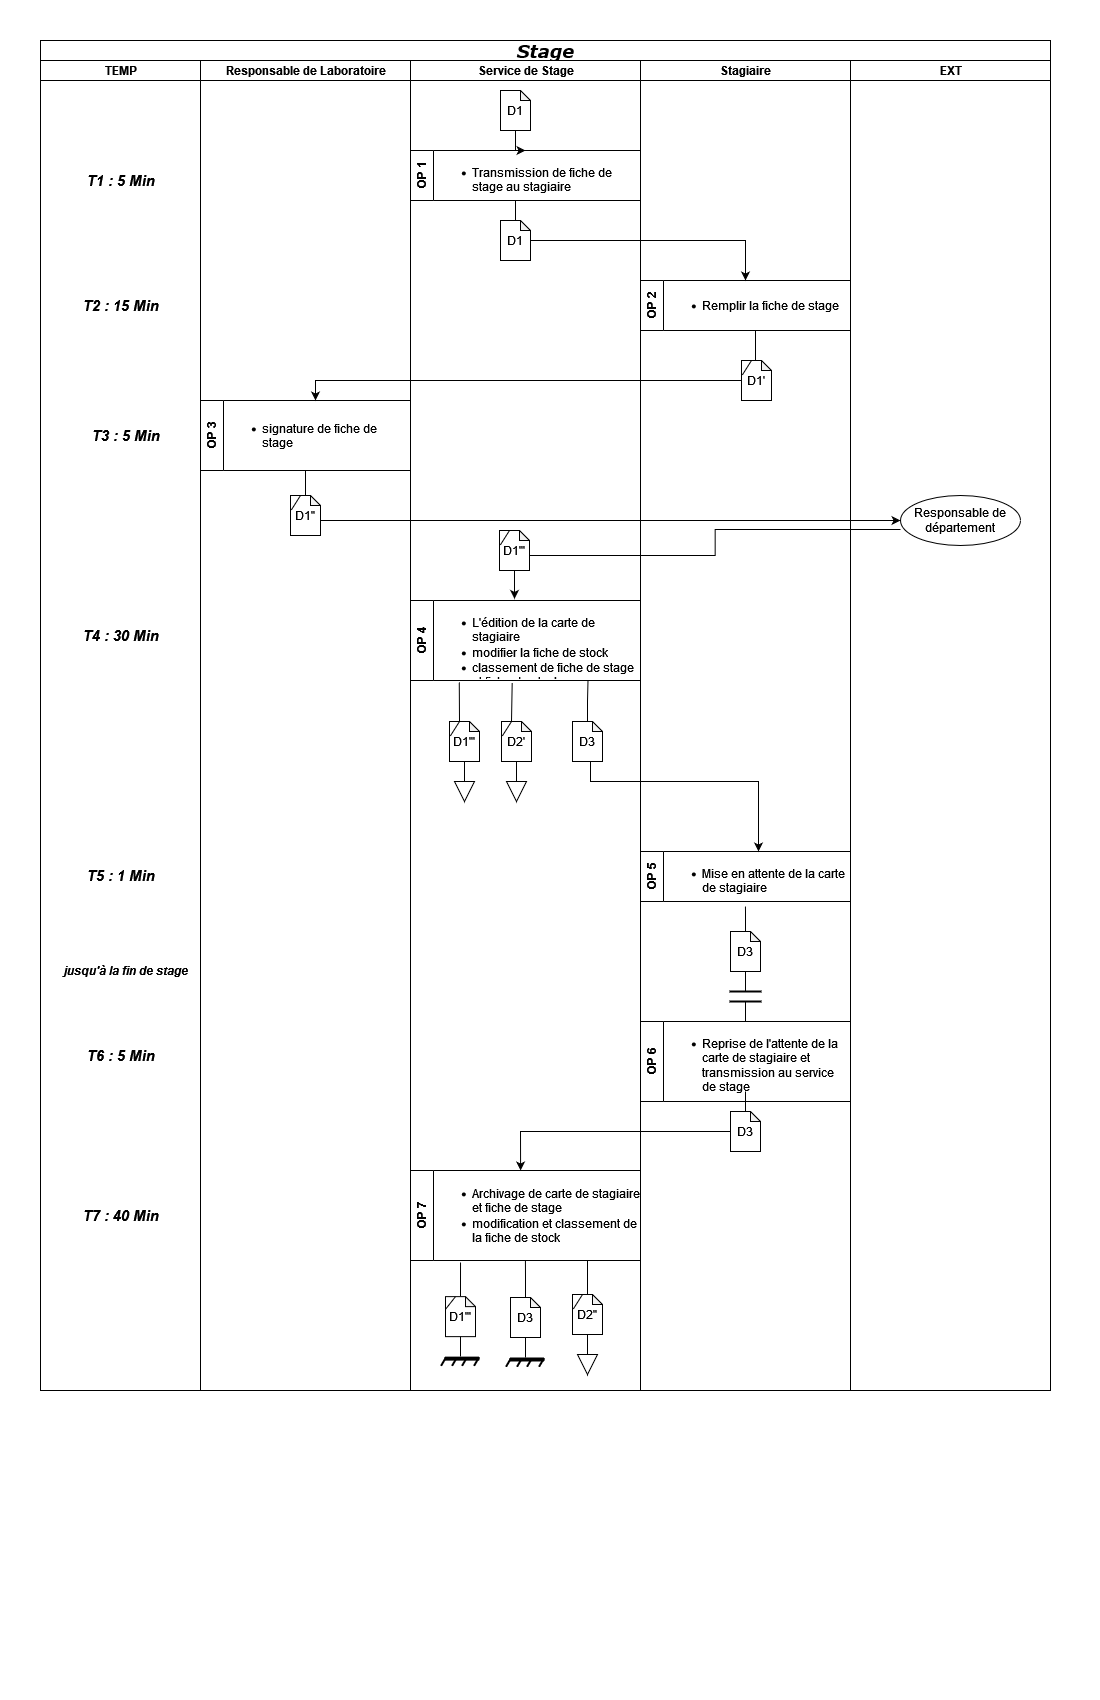
\includegraphics[width=1\textwidth]{chapter/Study of the Existing/EP/stage.png}
\subsubsection*{Description des documents}
\begin{itemize}
    \item D1:Fiche de Stage vierge
    \item D1':Fiche de Stage rempli
    \item D1'':Fiche de Stage signé par Responsable de laboratoire
    \item D1''':Fiche de Stage signé par Responsable de département
    \item D2:Fiche de Stock
    \item D2':Fiche de Stock modifier
    \item D3:Carte Stagiaire
\end{itemize}

\subsubsection*{Procédure n°2}
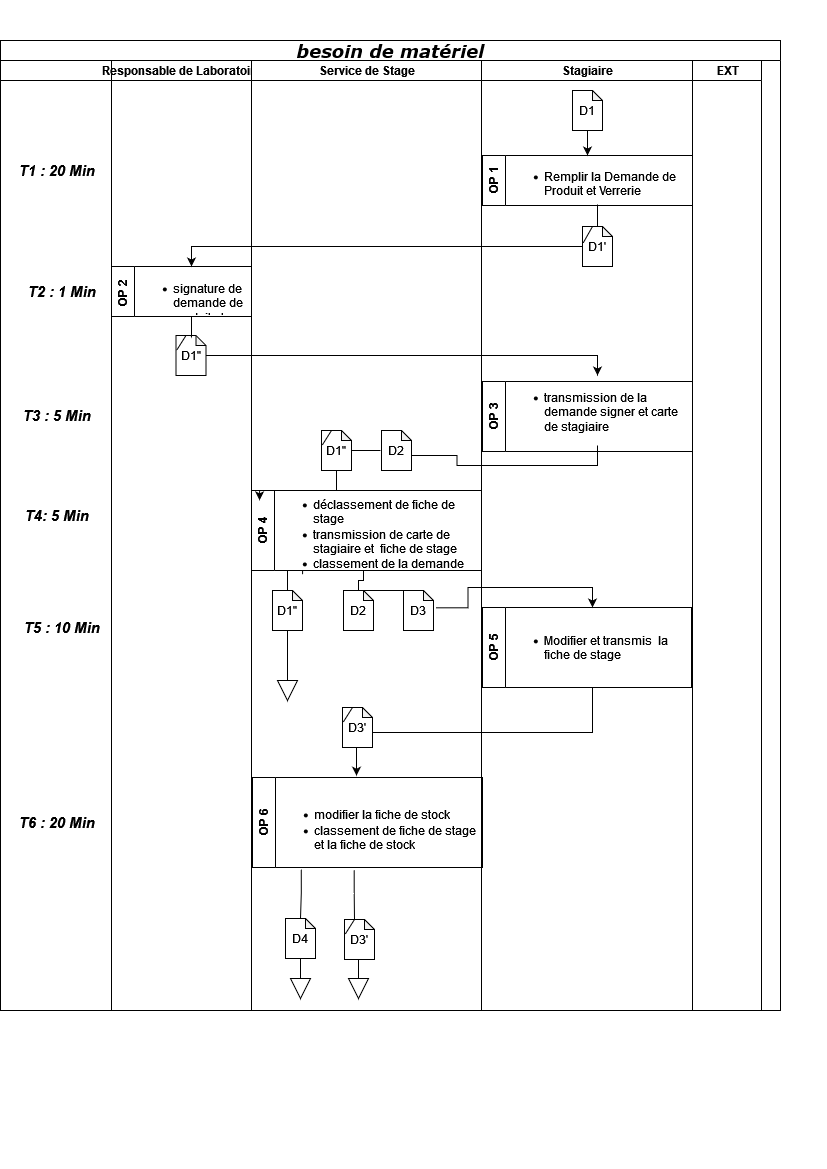
\includegraphics[width=1\textwidth]{chapter/Study of the Existing/EP/besoins.png}
\subsubsection*{Description des documents}
\begin{itemize}
    \item D1:Demande de Produit et Verrerie vierge 
    \item D1':Demande de Produit et Verrerie rempli
    \item D1'':Demande de Produit et Verrerie et signie
    \item D2:carte stagiaire
    \item D3:fiche de stage
    \item D3'':fiche de stage modifier
    \item D4:fiche de stock modifier
\end{itemize}

\subsubsection*{Procédure n°3}
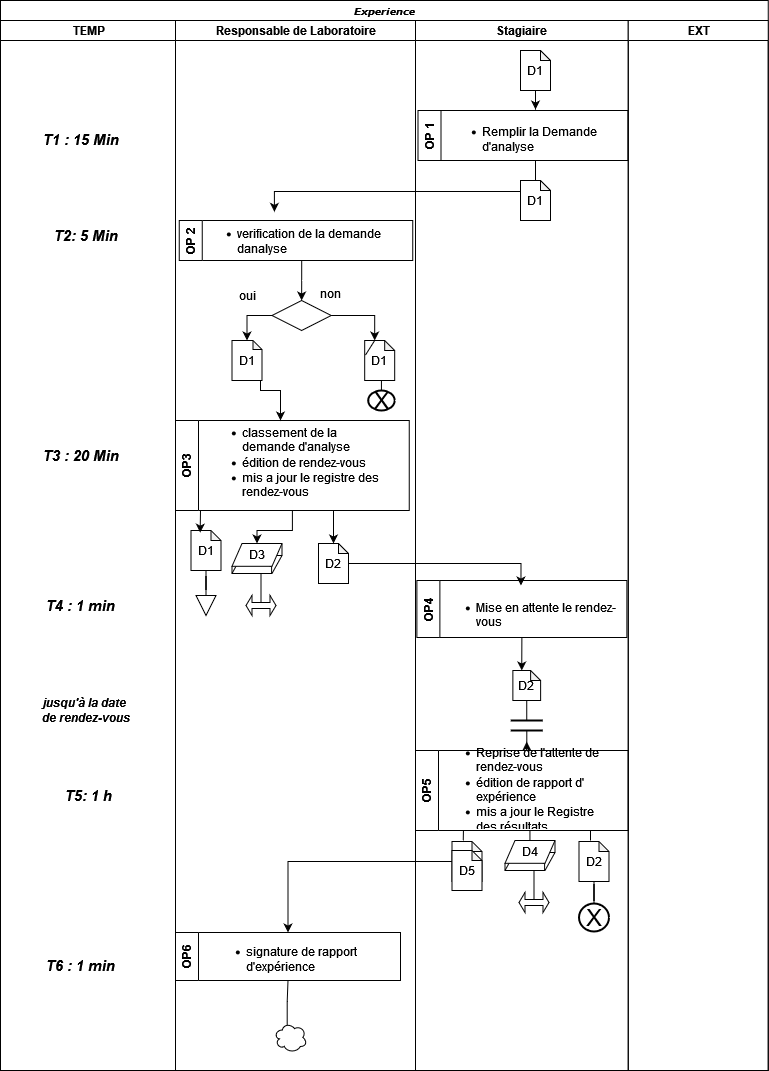
\includegraphics[width=1\textwidth]{chapter/Study of the Existing/EP/experience1.png}
\newpage
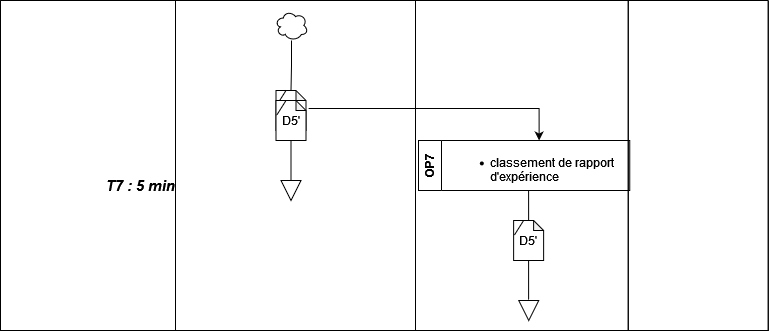
\includegraphics[width=1\textwidth]{chapter/Study of the Existing/EP/experience2.png}
\subsubsection*{Description des documents}
\begin{itemize}
    \item D1:demmand d'analyse
    \item D1':demmand d'analyse refuse
    \item D2:rende-vous
    \item D3:Registre des rende-vous
    \item D4:Registre des résultats
    \item D5:Rapport de expérience
    \item D5':Rapport de expérience signé
\end{itemize}


\subsubsection*{Procédure n°4}
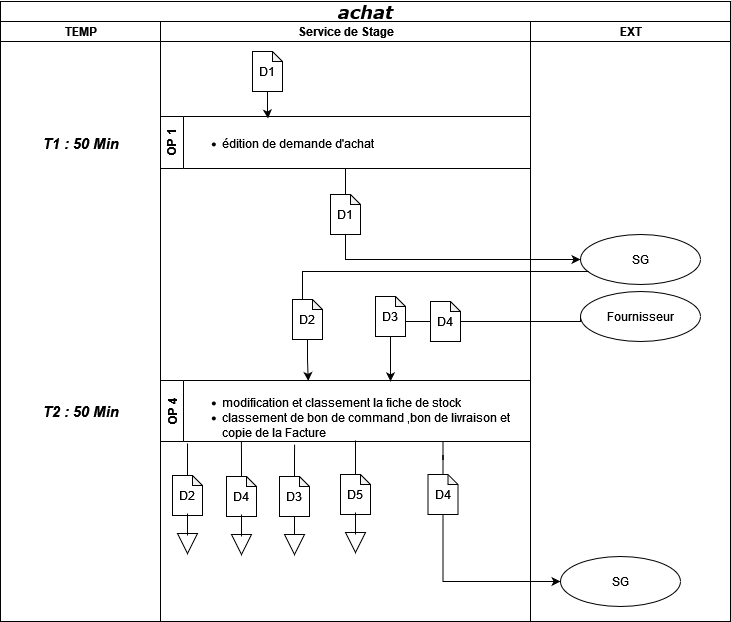
\includegraphics[width=1\textwidth]{chapter/Study of the Existing/EP/achat.png}
\subsubsection*{Description des documents}
\begin{itemize}
    \item D1:Demande d'achat
    \item D2:copie de Bon de Command
    \item D3:Bon de Livraison
    \item D4:Facture
    \item D5:Fiche de Stock modifier
\end{itemize}

\subsubsection*{Procédure n°5}
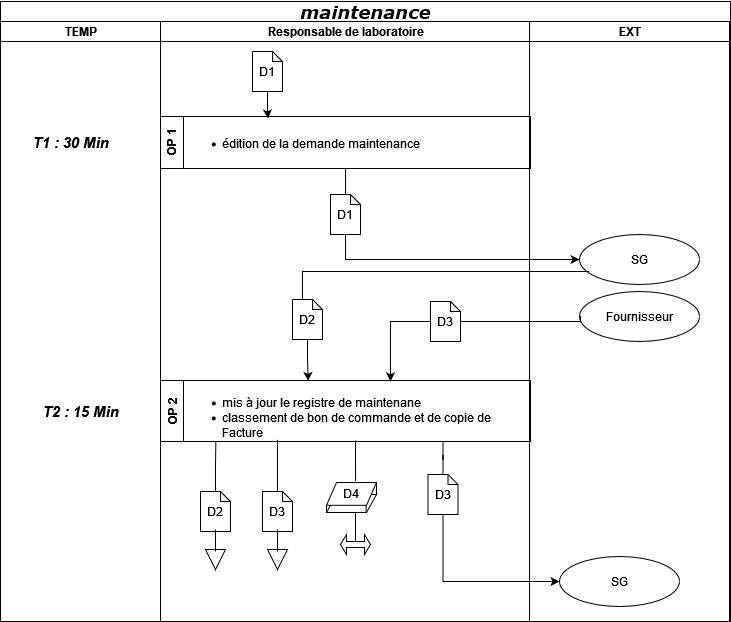
\includegraphics[width=1\textwidth]{chapter/Study of the Existing/EP/maintenance.png}
\subsubsection*{Description des documents}
\begin{itemize}
    \item D1:Demande de Maintenance
    \item D2:copie de Bon de Command
    \item D3:Facture
    \item D4:Registre de Maintenance
\end{itemize}

\subsubsection*{Procédure n°6}
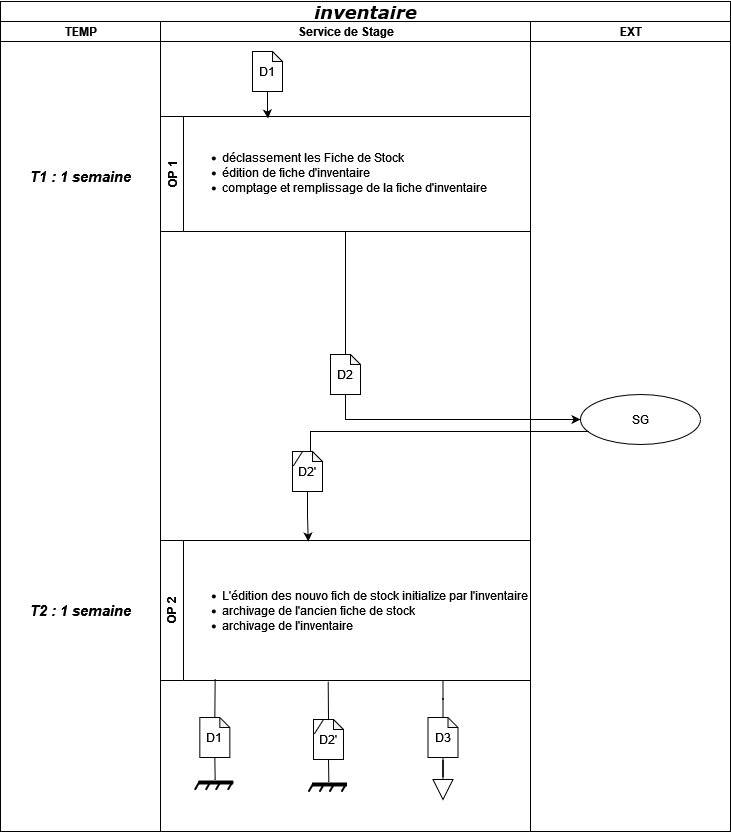
\includegraphics[width=1\textwidth]{chapter/Study of the Existing/EP/inventaire.png}
\subsubsection*{Description des documents}
\begin{itemize}
    \item D1:Fiche de stock
    \item D2:Fiche d'Inventaire
    \item D2':Fiche d'Inventaire signe
    \item D3:Nouvo Fiche de stock
\end{itemize}

\section{La grille d’information}
\subsection{Définition}
La grille d'information est la collecte de toutes les données récoltées à partir
des documents.
Elle se présente sous forme d'un tableau comportant en ligne les informations
des documents, fichiers registre correspondants.
Les lignes représentent les rubriques et les colonnes sont les documents
étudies.
\subsection{Les symboles utilisés}

\begin{table}[ht]
    \begin{tabularx}{\textwidth}{|X|X|}
    
    \hline
    \textbf{Symbole}    & \textbf{Désignation}   \\
    \hline
    \textbf{*}     &  Prévue porteuse (pp)  \\
    \hline
    \textbf{+}     &  Prévue porteuse (npp)  \\
    \hline
    \textbf{-}     &  Prévue non porteuse (pnp) \\
    \hline
    \end{tabularx}
    \end{table}
\subsection{Liste des documents utilisé}
\csvreader[longtable=|l|c|c|c|c|c|c|c|c|c|c|c|c|,
  table head=\caption{La grille d’information.\label{tab:La grille d’information.}}\\ \hline
  \bfseries doc&\bfseries FSG&\bfseries CS &\bfseries FSK &\bfseries DPV &\bfseries DAN &\bfseries RV &\bfseries RE &\bfseries DACH &\bfseries DM &\bfseries FI &\bfseries RRS &\bfseries RM \\ \endfirsthead \hline ,
  late after line=\\,table foot=\hline,
]{chapter/Study of the Existing/la_grille.csv}{1=\doc,2=\FSG,3=\CS,4=\FSK,5=\DPV,6=\DAN,7=\RV,8=\RE,9=\DACH,10=\DM,11=\FI,12=\RRS,13=\RM}{\doc&\FSG&\CS&\FSK&\DPV&\DAN&\RV&\RE&\DACH&\DM&\FI&\RRS&\RM}

\subsection{Analyse de la grille}
    \begin{table}[ht]
        \begin{tabularx}{\textwidth}{|X|X|X|X|X|}
        
            \hline
             & \textbf{PP}    & \textbf{PNP} & \textbf{NPP} & \textbf{TOTAL}   \\
            \hline
            \textbf{Utilisation} & 00 & 03 & 197 & 200  \\
            \hline
            \textbf{Symbole} & - & + & * &  \\
            \hline
            \textbf{Percentage} & 00\% & 98.5\% & 1.5\% & 100\% \\
            \hline
        \end{tabularx}
    \end{table}

\subsection{Description graphique}
    \begin{figure}[H]
        \centering
        \begin{tikzpicture}
            \pie[
                color = {green!60!black, yellow!90!black, blue!60}, 
                text = inside,
                explode = 0.1]{98.5 / PNP, 1.5 / NPP}
        \end{tikzpicture}
        \caption{Description graphique d'Analyse de la grille }
    \label{fig:piechart}
    \end{figure}
\subsection{Conclusion}
Après l’analyse de la grille nous somme arrivé a déduire que les documents de système existant ont une bonne conception avec une pourcentage de 98.5\% 
des rubrique prévue porteuse et 1.5\% des rubrique prévue non porteuse que nous allons l’améliorer dont le nouveaux système.
\section{Codification existante}
\subsection{Définition}
La codification implique d'attribuer des codes ou des identifiants uniques à différentes parties d'un document ou à des types spécifiques de données.\\
 Ces codes peuvent être sous forme de chiffres, de lettres, de combinaisons de caractères ou d'autres symboles conventionnels.\\
 Les systèmes de codification sont généralement bien définis et normalisés pour garantir la cohérence et la fiabilité des informations codées.
 \subsection{Déférentes type de la codification }
 \begin{enumerate}
    \item Codification séquentielle: Dans cette codification l'information est codée
par un numéro séquentiel.
    \item Codification par tranche: Consiste à réserver des codes à des catégories
d'objets, à l'intérieur de chaque tranche les objets sont codifiés de façon
séquentielle.
    \item Codification articulee : Les codes sont découpés en plusieurs zones dites
    « Descripteurs » dont chacune à un sens particulier.
    \item Codification hiérarchique (à niveau): C'est un cas particulier de la
    codification articulée. Les descripteurs sont des niveaux dont chacun
    représente un ensemble d'objets.
    \item Codification mnémonique: Consiste à représenter le nom de l'objet par un
    petit nombre de caractères qui rappelle l'objet. Doit être simple et non
    ambiguë.
 \end{enumerate}
\subsection{La codification utilisée par le système actuel}
 \begin{itemize}
    \item matricule chercheur: Codification articulee 
    C’est un code composé de 2 champ et de 12 caractères, 2 premier caractère l année et les 2 suivante l année  et le rest séquentiel \\
    example: 171731046640
    \item code appareil: Codification articulee 
    est un code composé de 2 champ abréviation de nom  d'appareil et le numero séquentiel de l'appareil
    \item code laboratoire: Codification séquentielle 
    example: 15,16
 \end{itemize}
 \section{Diagnostique}
Durant la période du stage il a été constaté que quelques problèmes sont
présents sur le plan organisationnel et technique après des entretiens avec les
acteurs.
\subsection{Critiques et suggestions}
\subsubsection{Les critiques:}
\begin{itemize}
    \item Le traitement manuel des taches comme l'edition des document\dots
    \item Manque de codefication des document, les experience \dots
    \item Risque d'erreurs En raison de la saisie manuelle des données, il existe un risque accru d'erreurs humaines telles que des fautes de frappe ou des omissions.
    \item La traçabilité des échantillons, des expériences et des produits chimiques peut être difficile à garantir avec un système manuel.
    \item Difficulté de suivi des stocks, La gestion des niveaux de stock et des commandes de produits chimiques peut être complexe et sujette à des erreurs.
    \item Limitations dans la planification des rendez-vous, La planification des rendez-vous peut être difficile à gérer efficacement sans un système automatisé.
\end{itemize}
\subsubsection{Suggestion:}
\begin{itemize}
    \item Informatisation des taches manuel
    \item codefication des document 
    \item  Mettre en place un système de gestion des stocks et de rendz-vous
    \item traçabilité des échantillons et des produits
\end{itemize}